\section{Struktura projektu}

Struktura projektu, a wraz z nią struktura repozytorium, odzwierciedla wyraźny podział na część software'ową (kompilator naszego języka programowania) oraz hardware'ową (koprocesor zaimplementowany na układzie FPGA). Dodatkowo, dokumentacja do projektu jest również trzymana w repozytorium, co umożliwia łatwiejszą współpracę nad jej tworzeniem i pozwala na zarządzanie jej wersjami.

Część hardware'owa, związana z FPGA, ma niemalże płaską strukturę: mamy jeden moduł główny i kilka pomniejszych komponentów, które są do niego dołączone (jako osobne części układu zaimplementowane są jego wyróżnione składowe, takie jak stos, pamięć ram czy moduł UART). Każdy z komponentów umieszczony jest w oddzielnym pliku.

Część software'owa jest w pełni autonomicznym projektem języka Haskell, budowanym systemem budowania Cabal. Narzuca to pewną strukturę plików i katalogów (w Haskellu tworzone są hierarchiczne moduły poprzez umieszczanie plików w odpowiednich ścieżkach folderów). Projekt podzielony jest na części związane z etapami kompilacji programów w naszym języku, w szczególności na dwa główne moduły: \texttt{Parser} i \texttt{CodeGen}, które z kolei podzielone są na bardziej szczegółowe submoduły. Dokładna struktura plików i katalogów została przedstawiona na rysunku \ref{fig:file-structure}.

\begin{figure}
  \begin{center}
    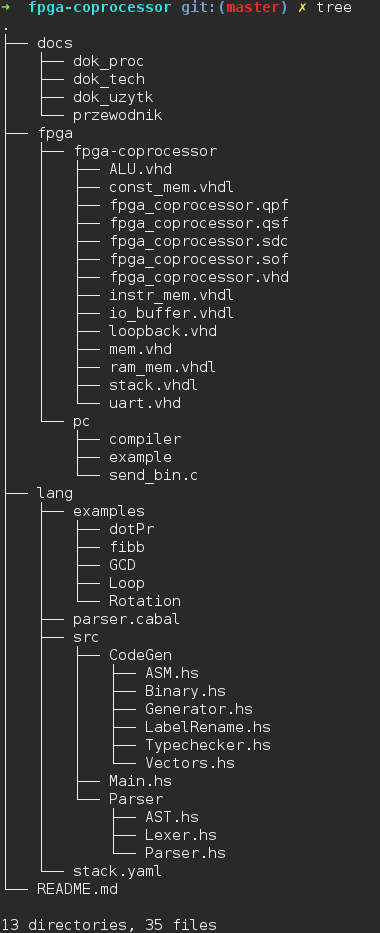
\includegraphics[scale=0.5]{images/file_structure.png}
    \caption{Struktura plików w projekcie jako wynik polecenia \texttt{tree} w systemie Linux.}
    \label{fig:file-structure}
  \end{center}
\end{figure}

\section{Porady dotyczące budowania}

Zwykły użytkownik systemu nie musi zajmować się jego budowaniem, jednak programista, pragnący rozwijać system, musi zapoznać się ze specyfiką budowania projektów języka Haskell w systemie Cabal oraz języka VHDL w środowisku Quartus.

\subsection{Haskell}
Cały projekt haskellowy mieści się w katalogu \texttt{lang}. Pierwszą rzeczą, na którą należy zwrócić uwagę jest plik \texttt{parser.cabal}. Jest to plik opisujący projekt Cabala, który służy nam m.in. do określania zależności projektu wraz z ich wersjami, dostarczania informacji o projekcie, ustawiania globalnych opcji kompilacji dla całego projektu, czy włączania rozszerzeń języka Haskell na poziomie projektu. W pliku tym możemy zdecydować, czy projekt ma być budowany jako biblioteka (\textit{library}) czy wykonywalny program (\textit{executable}). Możemy również, jak w przypadku naszego projektu, zbudować projekt na obydwa sposoby. Dla obydwu rodzajów budowania podajemy katalogi, w których kompilator ma szukać plików źródłowych (\texttt{hs-source-dirs}), opcje kompilatora (\texttt{Ghc-Options}) i zależności (\texttt{build-depends}).

Zależności są polem, na które warto zwrócić szczególną uwagę. W przeciwieństwie do systemów budowania języka Java, takich jak Maven, Cabal nie ściąga archiwów \texttt{.jar} z bibliotekami. Ściąga jedynie źródła, które potem kompiluje. Tworzy to pewne problemy z wersjami bibliotek (wyobraźmy sobie sytuację, w której biblioteka $A$ wymaga biblioteki $B$ w wersji 0.1 oraz biblioteki $C$ w wersji 0.2, a z kolei biblioteka $B$ wymaga biblioteki $C$ w wersji 0.3 --- problemy z wersjami bibliotek są powszechne przy stosowaniu Cabala), które możemy próbować obchodzić przez wymuszanie konkretnych wersji bibliotek lub ich przedziałów. W naszym projekcie jednak wybór padł na używanie wszystkich bibliotek w ich najnowszych wersjach, więc żadne wersje nie są sztucznie wymuszane. Jest to możliwe również dzięki zastosowaniu technologii \textit{sandboxów}. Zamiast instalować wszystkie biblioteki globalnie do systemu (co potencjalnie rodzi konflikty, jeśli mamy więcej niż jeden projekt), instalujemy je do osobnego środowiska umieszczonego w osobnym folderze, które możemy łatwo usunąć i odtworzyć w razie problemów.

Po zainstalowaniu projektu poleceniem \texttt{cabal install} utworzy się folder \texttt{dist}, w którym można znaleźć pliki wykonywalne i biblioteki utworzone podczas budowania. Popularną praktyką wśród programistów Haskella jest usuwanie katalogu \texttt{dist} w razie problemów z budowaniem i \texttt{.cabal-sandbox} w razie problemów z wersjami pakietów.

\subsection{FPGA}

Projekt FPGA jest utworzony w środowisku Quartus II firmy Altera, które automatyzuje budowanie projektu przez dostarczenie zintegrowanego środowiska do projektowania i syntezy układów. Kompilacja odbywa się za pomocą graficznego interfejsu i nie wymaga szczegółowego opisywania. W razie problemów z kompilacją Altera dostarcza obszerną dokumentację do środowiska Quartus. Ważnym plikiem jest \texttt{fpga\_coprocessor.qsf}, który zawiera przypisania pinów (\textit{pin assignments}) dla projektu. W przypadku budowania projektu dla innej płytki, niż Altera De0-Nano, należy zmienić plik tak, by nazwy pinów odpowiadały tym, które faktycznie są dostępne na płytce. Jest to o tyle istotne, że w przypadku rozszerzania układu może zajść konieczność użycia większej płytki (z większą ilością elementów logicznych i szybszym wejściem-wyjściem).

\subsection{Komunikacja}

Aby skompilować prosty program do obsługi komunikacji z koprocesorem, który można znaleźć w katalogu \texttt{fpga/pc} wystarczy zwyczajny kompilator języka C. Przy tworzeniu projektu wykorzystano kompilator GCC w wersji 5.1, choć każdy kompilator obsługujący standard C99 wystarczy do skompilowania programu. Przykładowe polecenie to: \texttt{gcc -o sender sender.c}. Dodatkowo, komunikacja odbywa się przez port szeregowy, więc trzeba zadbać, by urządzenie w systemie, jako które widoczny jest nasz port, było faktycznie rozpoznawane przez system jako port szeregowy. Służy temu polecenie \texttt{setserial}, dostępne w systemach linuksowych po zainstalowaniu pakietu o tej samej nazwie. Przykładowo, używając systemu Fedora 22 musimy wydać polecenie: \texttt{sudo dnf install setserial \&\& sudo setserial -g /dev/ttyUSB0}. W powyższych instrukcjach bazujemy na założeniu, że do komunikacji używana jest przejściówka USB-UART. Jeśli do rozwoju systemu zostanie użyty inny sposób podłączenia (np. bezpośrednio do pinów GPIO na urządzeniach typu Arduino bądź Raspberry Pi), nazwa urządzenia może ulec zmianie.
